\documentclass[12pt,a4paper]{article}
\usepackage[utf8]{inputenc}
\usepackage[english]{babel}
\usepackage{graphicx}
\usepackage{amsmath,amssymb,amsfonts}
\usepackage{booktabs}
\usepackage{multirow}
\usepackage{float}
\usepackage{hyperref}
\usepackage{subcaption}
\usepackage{xcolor}
\usepackage{geometry}
\usepackage{listings}
\usepackage{csquotes}
\usepackage{algorithm}
\usepackage{algpseudocode}
\usepackage{tikz}

\geometry{margin=1in}


% Directory for output
\makeatletter
\@latex@warning@no@line{Creating output directory 'build' if it doesn't exist}
\makeatother
\immediate\write18{mkdir -p build}

% Custom colors for code listings
\definecolor{codegreen}{rgb}{0,0.6,0}
\definecolor{codegray}{rgb}{0.5,0.5,0.5}
\definecolor{codepurple}{rgb}{0.58,0,0.82}
\definecolor{backcolour}{rgb}{0.95,0.95,0.92}
\definecolor{alexuniblue}{rgb}{0.0, 0.27, 0.53} % Alexandria University Blue

% Listings style for code
\lstdefinestyle{mystyle}{
    backgroundcolor=\color{backcolour},   
    commentstyle=\color{codegreen},
    keywordstyle=\color{magenta},
    numberstyle=\tiny\color{codegray},
    stringstyle=\color{codepurple},
    basicstyle=\ttfamily\footnotesize,
    breakatwhitespace=false,         
    breaklines=true,                 
    captionpos=b,                    
    keepspaces=true,                 
    numbers=left,                    
    numbersep=5pt,                  
    showspaces=false,                
    showstringspaces=false,
    showtabs=false,                  
    tabsize=2
}
\lstset{style=mystyle}

% Use a more pseudocode style for listings
\lstdefinestyle{pseudocode}{
    backgroundcolor=\color{white},
    commentstyle=\color{codegreen},
    keywordstyle=\color{blue},
    numberstyle=\tiny\color{codegray},
    stringstyle=\color{codepurple},
    basicstyle=\ttfamily\normalsize,
    breakatwhitespace=false,
    breaklines=true,
    captionpos=b,
    keepspaces=true,
    numbers=none,
    numbersep=5pt,
    showspaces=false,
    showstringspaces=false,
    showtabs=false,
    tabsize=2,
    frame=none
}

\title{Speech Emotion Recognition}
\author{
Youssif Khaled Ahmed (21011655) \\ 
\and
Esmail Mahmoud Hassan (21010272) \\
\and
Ahmed Ayman Ahmed (21010048)
}
\date{\today}

\begin{document}

% Custom title page
\begin{titlepage}
    \centering
    \vspace*{1cm}
    {\Large\textbf{Alexandria University}\\}
    {\large Faculty of Engineering\\}
    {\large Computer and Systems Engineering Department\\}
    \vspace{1.5cm}
    
    % \includegraphics[width=0.3\textwidth]{faculty.jpg}\\
    \vspace{1.5cm}
    
    {\huge\bfseries\color{alexuniblue} Speech Emotion Recognition\\}
    \vspace{1.5cm}

    \begin{tabular}{l@{\hspace{4em}}r}
        \textbf{Youssif Khaled Ahmed} & \textbf{21011655} \\
        \textbf{Esmail Mahmoud Hassan} & \textbf{21010272} \\
        \textbf{Ahmed Ayman Ahmed} & \textbf{21010048} \\
    \end{tabular}
    \vspace{1.5cm}
    
    {\large Course: CSE: Pattern Recognition\\}
    {\large Instructors: Prof. Dr. Marwan Torki, Eng. Ismail El-Yamany\\}
    \vspace{1cm}
    
    
    \vspace{4.5em}
    \begin{abstract}
        This report presents a comprehensive analysis of Speech Emotion Recognition (SER) systems, focusing on feature extraction techniques and comparative performance of various CNN architectures. We implement both 1D and 2D convolutional networks for emotion classification using the CREMA dataset, exploring different activation functions (ReLU, SiLU, ELU) and learning rates. Our experiments demonstrate the effectiveness of combined feature spaces and provide insights into the most confusing emotion classes in speech recognition.
    \end{abstract}
    
\end{titlepage}

    \clearpage
    
\tableofcontents
\clearpage

% Include all sections
\section{Introduction}

Speech is the most natural way of expressing ourselves as humans. It is only natural then to extend this communication medium to computer applications. Speech emotion recognition (SER) systems are collections of methodologies that process and classify speech signals to detect embedded emotions. These systems have numerous applications in human-computer interaction, customer service analysis, mental health monitoring, and entertainment.

SER presents unique challenges because emotional expressions in speech vary significantly across individuals, cultures, and contexts. The acoustic features that convey emotion can be subtle and often overlap with other speech characteristics. This assignment explores different approaches to SER, focusing on:

\begin{itemize}
    \item Extracting relevant features from speech signals using both time and frequency domain representations
    \item Developing and comparing 1D and 2D CNN architectures for emotion classification
    \item Analyzing the effects of different learning rates and activation functions on model performance
    \item Identifying confusing emotion classes and investigating the causes of misclassification
\end{itemize}

We utilize the CREMA dataset, which contains acted emotional speech recordings from multiple speakers expressing six basic emotions: sadness, anger, disgust, fear, happiness, and neutral. Our goal is to build effective SER models and provide insights into the relative performance of different feature extraction and classification techniques. 
\section{Dataset Understanding and Visualization}

\subsection{CREMA Dataset}

For this project, we used the CREMA (Crowd-sourced Emotional Multimodal Actors) dataset, which is widely used in speech emotion recognition research. The dataset consists of audio recordings from 91 actors (48 male, 43 female) with diverse ethnic backgrounds, expressing six basic emotions:

\begin{itemize}
    \item Sadness (SAD)
    \item Anger (ANG)
    \item Disgust (DIS)
    \item Fear (FEA)
    \item Happiness (HAP)
    \item Neutral (NEU)
\end{itemize}

The dataset contains 7,442 audio clips in total, with each clip labeled with the corresponding emotion. The filenames in the CREMA dataset follow a specific format that encodes information about the speaker and emotion: 

\texttt{[ActorID]\_[Sentence]\_[Emotion]\_[Intensity].wav}

For example, \texttt{1001\_AAA\_SAD\_XX.wav} represents a recording from Actor 1001, speaking sentence AAA with sad emotion at regular intensity (XX).

\subsection{Audio Waveform Visualization}

To better understand the dataset, we extracted and visualized sample audio waveforms from each emotion category. Figure \ref{fig:waveforms} shows example waveforms from each of the six emotion classes.
\begin{figure}[h]
    \centering
    \begin{subfigure}[b]{0.32\textwidth}
        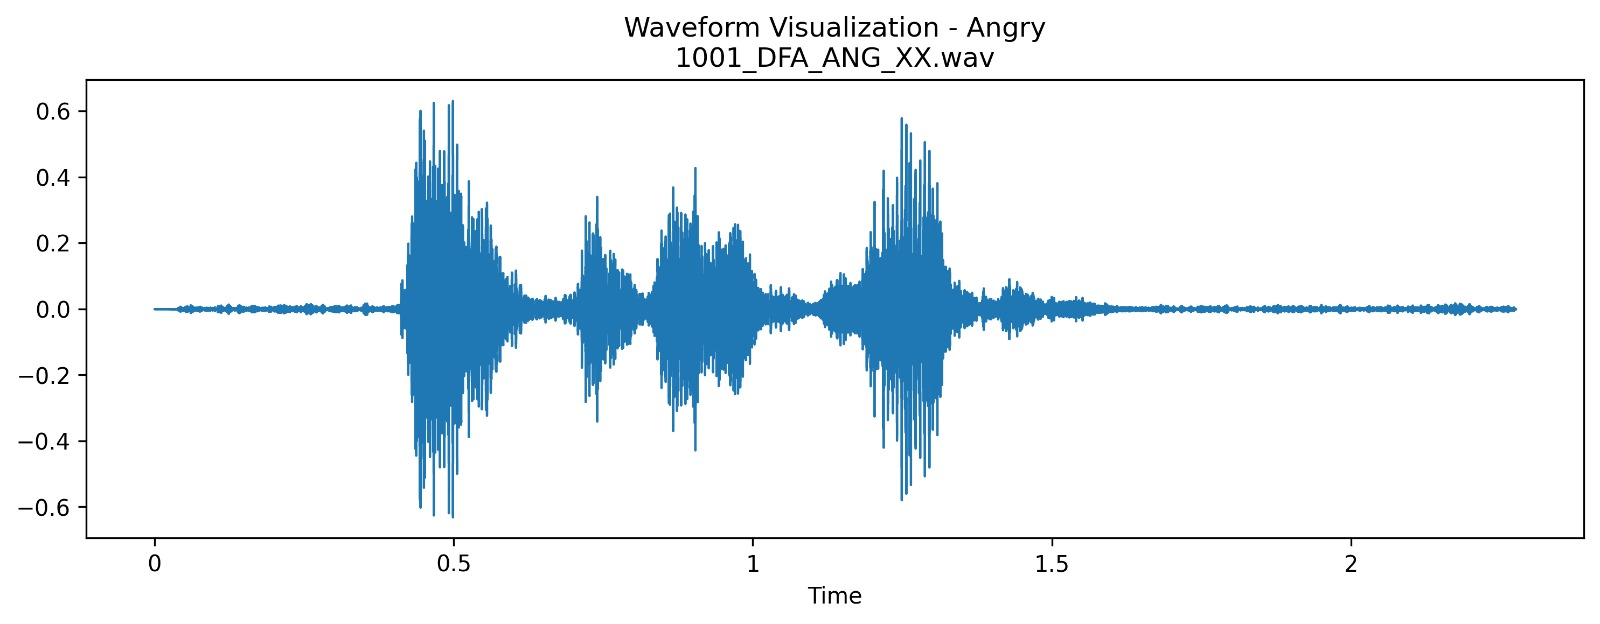
\includegraphics[width=\textwidth]{images/anger.jpeg}
        \caption{Anger}
    \end{subfigure}
    \begin{subfigure}[b]{0.32\textwidth}
        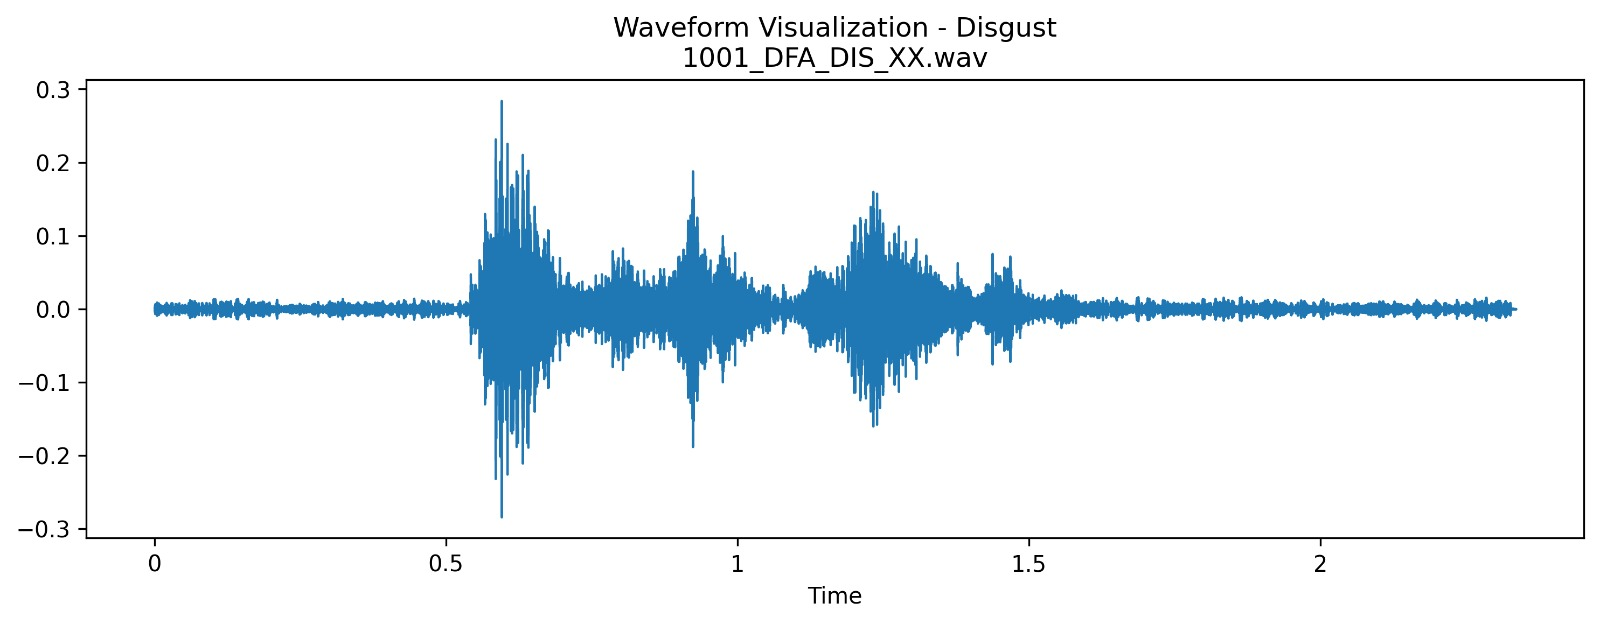
\includegraphics[width=\textwidth]{images/disgust.jpeg}
        \caption{Disgust}
    \end{subfigure}
    \begin{subfigure}[b]{0.32\textwidth}
        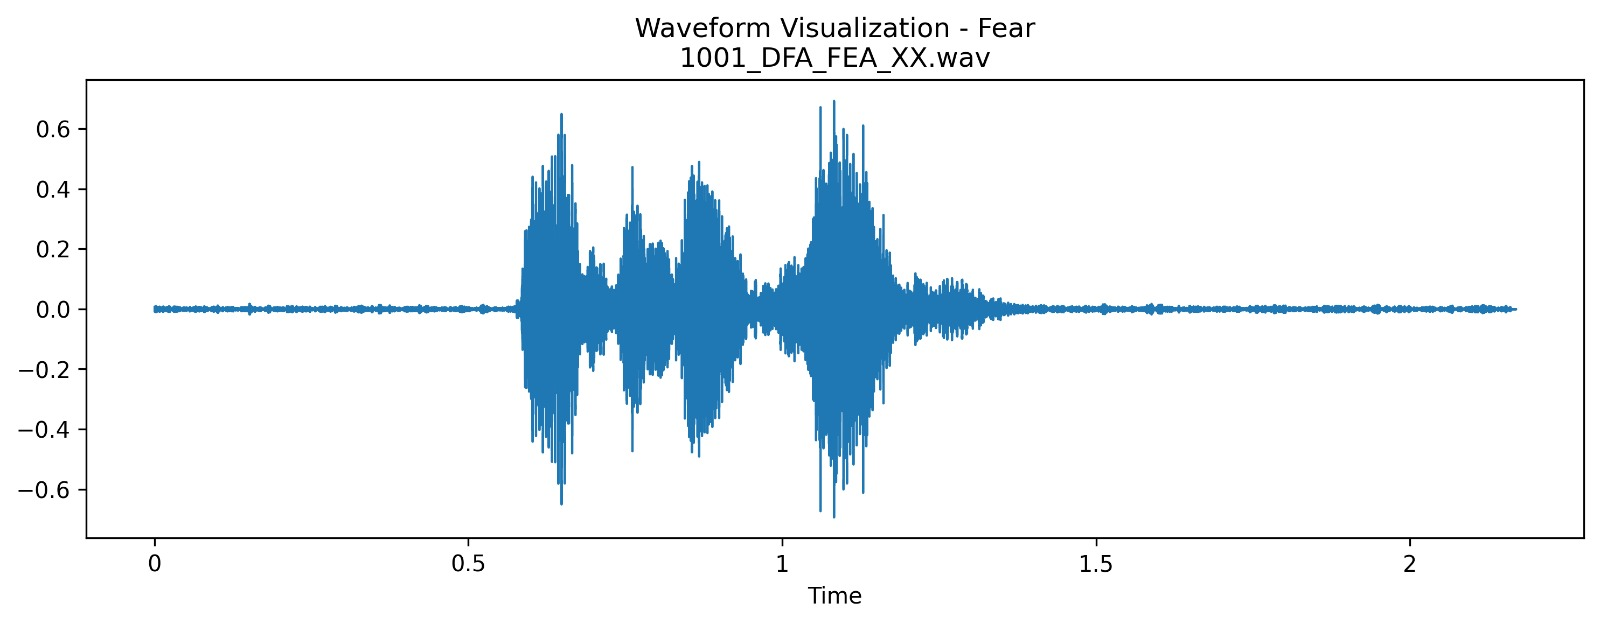
\includegraphics[width=\textwidth]{images/fear.jpeg}
        \caption{Fear}
    \end{subfigure}
    
    \begin{subfigure}[b]{0.32\textwidth}
        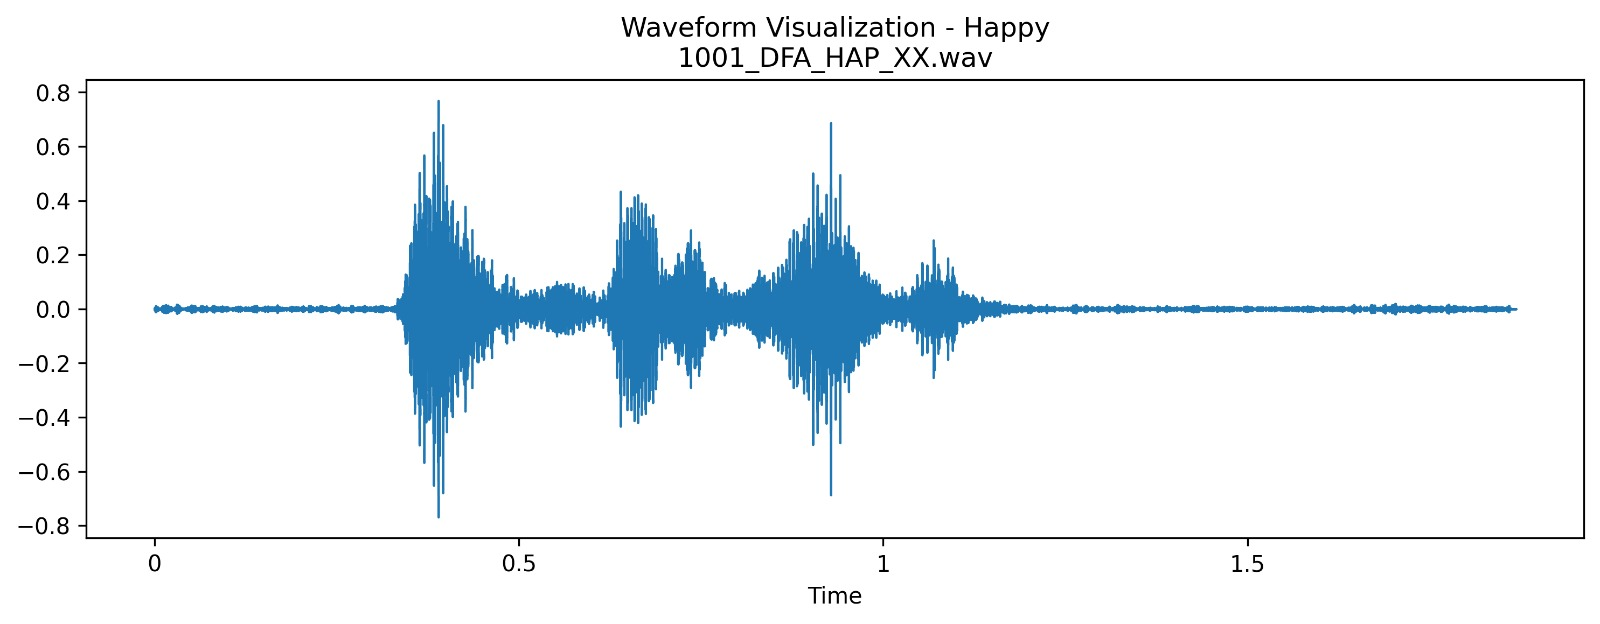
\includegraphics[width=\textwidth]{images/happy.jpeg}
        \caption{Happiness}
    \end{subfigure}
    \begin{subfigure}[b]{0.32\textwidth}
        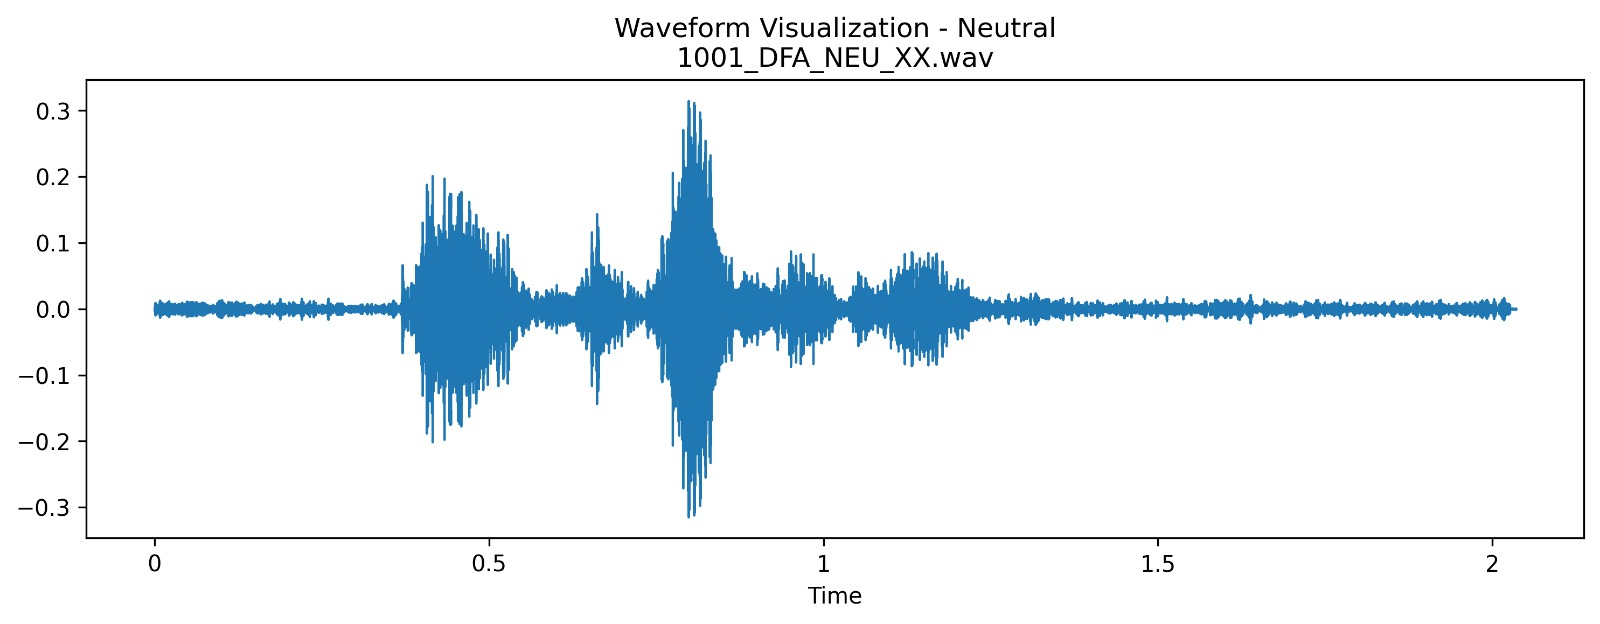
\includegraphics[width=\textwidth]{images/neutral.jpeg}
        \caption{Neutral}
    \end{subfigure}
    \begin{subfigure}[b]{0.32\textwidth}
        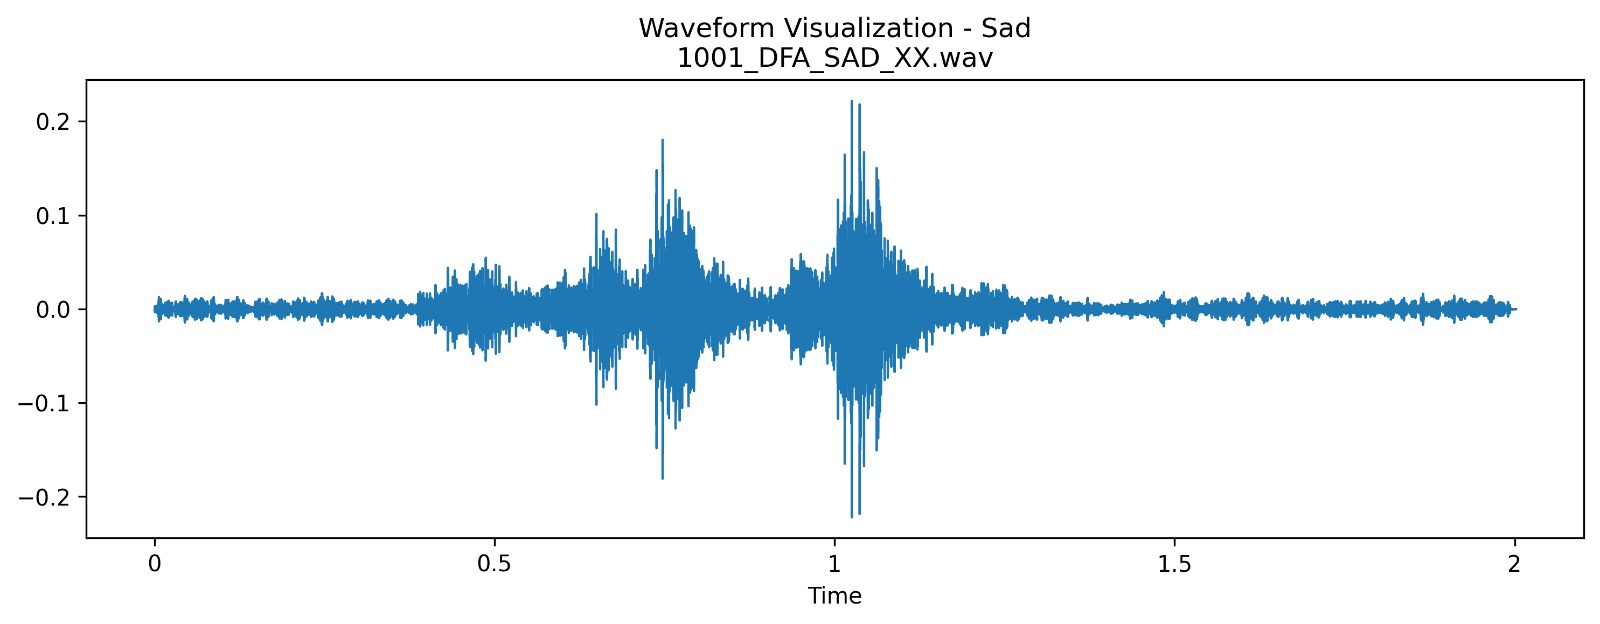
\includegraphics[width=\textwidth]{images/sad.jpeg}
        \caption{Sadness}
    \end{subfigure}
    \caption{Sample waveforms from the CREMA dataset for each emotion class. Notice the variations in amplitude patterns and signal density across different emotional expressions.}
    \label{fig:waveforms}
\end{figure}

\subsection{Audio Preprocessing}

Before feature extraction, we applied several preprocessing steps to prepare the raw audio data:

\begin{itemize}
    \item Conversion to mono channel: All stereo recordings were converted to mono by averaging the channels
    \item Resampling: All audio was resampled to 16kHz for consistency
    \item Voice Activity Detection (VAD): Applied to remove silence and improve signal-to-noise ratio
    \item Normalization: Z-score normalization was applied to standardize signal amplitude
\end{itemize}

These preprocessing steps ensured that our models would be learning from the emotional content rather than variations in recording quality or silence periods. 
\section{Feature Extraction}

We implemented two distinct approaches for feature extraction from the preprocessed audio signals: 1D spectral features and 2D mel spectrogram images. This dual-path approach allowed us to evaluate the effectiveness of different feature representations for emotion recognition.

\subsection{1D Spectral Features}

For the 1D feature space, we extracted a combination of time and frequency domain features that capture various acoustic properties relevant to emotion expression. Our feature vector included:

\begin{itemize}
    \item \textbf{Zero Crossing Rate (ZCR)}: The rate at which the signal changes from positive to negative or vice versa, capturing information about the frequency content and noisiness of the signal.
    
    \item \textbf{Chroma STFT}: A 12-element feature vector representing the spectral energy distribution across the 12 different pitch classes (C, C\#, D, etc.), which helps capture tonal content.
    
    \item \textbf{Mel-Frequency Cepstral Coefficients (MFCCs)}: 13 coefficients representing the short-term power spectrum of the sound on a mel scale, which approximates the human auditory system's response.
    
    \item \textbf{Root Mean Square (RMS) Energy}: A measure of the loudness or energy in the signal, capturing amplitude variations that often correlate with emotional intensity.
\end{itemize}

These features were extracted using frame-by-frame processing with a frame length of 512 samples and a hop length of 160 samples. The resulting feature matrix had 27 rows (feature channels) and 301 time frames, which served as input to our 1D CNN models.

\subsection{2D Mel Spectrogram Features}

For the 2D feature space, we converted the audio signals into mel spectrograms, which are visual representations of the spectrum of frequencies over time. The mel scale is a perceptual scale that better represents how humans perceive pitch.

\begin{itemize}
    \item FFT window size: 1024 samples
    \item Hop length: 256 samples
    \item Number of mel bands: 64
    \item Frequency range: Up to 10 kHz (as per paper recommendations)
\end{itemize}

The resulting spectrograms were then:
\begin{itemize}
    \item Converted to logarithmic scale to better represent human hearing perception
    \item Normalized to the range [0,1]
    \item Resized to a fixed dimension of 64×64 pixels to ensure uniform input size for the CNN
\end{itemize}

This process transformed each audio sample into an image-like representation where the x-axis represents time, the y-axis represents frequency (on the mel scale), and the pixel intensity represents the amplitude of a particular frequency at a given time.

Our dual feature extraction approach allowed us to compare the effectiveness of 1D spectral features and 2D spectrogram representations for emotion recognition, as well as to explore a combined approach that leverages both feature spaces. 
\section{Model Architecture}

We implemented three distinct CNN architectures for speech emotion recognition: a 1D CNN for spectral features, a 2D CNN for mel spectrogram images, and a combined model that leverages both feature spaces. This section describes the design of each architecture.

\subsection{1D CNN Architecture}

The 1D CNN is designed to process the time series of spectral features extracted from the audio signals. The architecture consists of three convolutional blocks followed by a global average pooling layer and a fully connected layer.

Each convolutional block in the 1D CNN includes:
\begin{itemize}
    \item 1D Convolutional layer with increasing filter sizes (128, 256, 512)
    \item Group Normalization for stable training
    \item Activation function (ReLU, SiLU, or ELU, depending on the experiment)
    \item Max Pooling layer with kernel size 2 and stride 2
    \item Dropout layer with dropout rate 0.3
\end{itemize}

\begin{lstlisting}[language=Python, style=pseudocode, caption=1D CNN Architecture (Pseudocode)]
class CNN1D:
    input: Spectral features with shape [batch_size, channels, time]
    
    ConvBlock1:
        Conv1D(in_channels=input_channels, out_channels=128, kernel_size=3, padding=1)
        GroupNorm(channels=128)
        Activation(ReLU/SiLU/ELU)
        MaxPool1D(kernel_size=2, stride=2)
        Dropout(p=0.3)
    
    ConvBlock2:
        Conv1D(in_channels=128, out_channels=256, kernel_size=3, padding=1)
        GroupNorm(channels=256)
        Activation(ReLU/SiLU/ELU)
        MaxPool1D(kernel_size=2, stride=2)
        Dropout(p=0.3)
    
    ConvBlock3:
        Conv1D(in_channels=256, out_channels=512, kernel_size=3, padding=1)
        GroupNorm(channels=512)
        Activation(ReLU/SiLU/ELU)
        MaxPool1D(kernel_size=2, stride=2)
        Dropout(p=0.3)
    
    GlobalAveragePooling1D()
    
    output: Feature vector of size 512
\end{lstlisting}

\subsection{2D CNN Architecture}

The 2D CNN processes mel spectrogram images and consists of four convolutional blocks followed by global average pooling and a fully connected layer.

Each convolutional block in the 2D CNN includes:
\begin{itemize}
    \item 2D Convolutional layer with increasing filter sizes (32, 64, 512, 1024)
    \item Group Normalization for stable training
    \item Activation function (ReLU, SiLU, or ELU, depending on the experiment)
    \item Max Pooling layer with kernel size (2,2) and stride 2
    \item Dropout layer with dropout rate 0.3
\end{itemize}

\begin{lstlisting}[language=Python, style=pseudocode, caption=2D CNN Architecture (Pseudocode)]
class CNN2D:
    input: Mel spectrogram with shape [batch_size, channels, height, width]
    
    ConvBlock1:
        Conv2D(in_channels=input_channels, out_channels=32, kernel_size=3x3, padding=1)
        GroupNorm(channels=32)
        Activation(ReLU/SiLU/ELU)
        MaxPool2D(kernel_size=2x2, stride=2)
        Dropout(p=0.3)
    
    ConvBlock2:
        Conv2D(in_channels=32, out_channels=64, kernel_size=3x3, padding=1)
        GroupNorm(channels=64)
        Activation(ReLU/SiLU/ELU)
        MaxPool2D(kernel_size=2x2, stride=2)
        Dropout(p=0.3)
    
    ConvBlock3:
        Conv2D(in_channels=64, out_channels=512, kernel_size=3x3, padding=1)
        GroupNorm(channels=512)
        Activation(ReLU/SiLU/ELU)
        MaxPool2D(kernel_size=2x2, stride=2)
        Dropout(p=0.3)
    
    ConvBlock4:
        Conv2D(in_channels=512, out_channels=1024, kernel_size=3x3, padding=1)
        GroupNorm(channels=1024)
        Activation(ReLU/SiLU/ELU)
        MaxPool2D(kernel_size=2x2, stride=2)
        Dropout(p=0.3)
    
    GlobalAveragePooling2D()
    
    output: Feature vector of size 1024
\end{lstlisting}

\subsection{Combined Model Architecture}

The combined model integrates both 1D and 2D feature paths. It processes spectral features using the 1D CNN path and mel spectrograms using the 2D CNN path, then concatenates the resulting feature vectors before passing them through a final fully connected layer for classification.

The combined model architecture:
\begin{itemize}
    \item Processes 1D spectral features through the 1D CNN path
    \item Processes 2D mel spectrograms through the 2D CNN path
    \item Concatenates the output feature vectors (512 features from 1D CNN, 1024 features from 2D CNN)
    \item Passes the combined features through a fully connected block with layer normalization and dropout
    \item Outputs emotion class probabilities
\end{itemize}

\begin{lstlisting}[language=Python, style=pseudocode, caption=Combined Model Architecture (Pseudocode)]
class CombinedModel:
    inputs:
        x_1d: Spectral features with shape [batch_size, channels, time]
        x_2d: Mel spectrogram with shape [batch_size, channels, height, width]
    
    # 1D CNN Path
    features_1d = CNN1D(x_1d)    # Output: [batch_size, 512]
    
    # 2D CNN Path  
    features_2d = CNN2D(x_2d)    # Output: [batch_size, 1024]
    
    # Feature Fusion
    combined_features = Concatenate([features_1d, features_2d])    # [batch_size, 1536]
    
    # Classification Head
    FCLayer:
        Linear(in_features=1536, out_features=128)
        LayerNorm(128)
        Activation(ReLU/SiLU/ELU)
        Dropout(p=0.5)
        Linear(in_features=128, out_features=num_classes)
    
    output: Class probabilities [batch_size, num_classes]
\end{lstlisting}

\subsection{Alternative Architectures Explored}

In addition to our main architecture, we also experimented with:

\begin{itemize}
    \item \textbf{ResNet-based models}: We implemented ResNet-38 and ResNet-101 architectures for comparison, which showed different levels of overfitting (particularly ResNet-101 with validation accuracy of 0.41 vs. train accuracy of 0.7)
    
    \item \textbf{Modified input dimensions}: We standardized the 2D input size to 64×64.
    
    \item \textbf{Variable length input}: Instead of fixed-size inputs, we also experimented with variable-length audio processing, which achieved better results (62.2\% accuracy on the combined model) compared to fixed-size inputs (61.3\%).
    
    \item \textbf{Modified 1D feature extraction}: We experimented with a single-channel approach using mean over time for fixed size input, which achieved comparable accuracy in the combined model.
\end{itemize}

These explorations helped us understand the trade-offs between model complexity, feature representation, and performance in the SER task. 
\section{Experimental Setup}

\subsection{Data Splitting}

Following the assignment requirements, we split the CREMA dataset as follows:
\begin{itemize}
    \item Training and Validation: 70\% of the dataset
    \item Test: 30\% of the dataset
    \item Of the 70\% training and validation portion, 5\% was used for validation
\end{itemize}

This resulted in approximately 4,960 training samples, 260 validation samples, and 2,222 test samples. We used stratified sampling with a random seed of 42 to ensure a balanced distribution of emotion classes across all splits.

\begin{lstlisting}[language=Python, caption=Data Splitting Implementation]
# Train/Val/Test Split
train_val_files, test_files, train_val_labels, test_labels = train_test_split(
    all_wav_files, all_labels, test_size=0.30, random_state=config.RANDOM_SEED, 
    stratify=all_labels
)
val_split_proportion = 0.05 
train_files, val_files, train_labels, val_labels = train_test_split(
    train_val_files, train_val_labels, test_size=val_split_proportion, 
    random_state=config.RANDOM_SEED, stratify=train_val_labels
)
\end{lstlisting}

\subsection{Training Configuration}

We conducted extensive experiments with different model configurations, focusing on three key variables:
\begin{itemize}
    \item \textbf{Model Type}: 1D CNN, 2D CNN, or Combined Model
    \item \textbf{Activation Function}: ReLU, SiLU (Swish), or ELU
    \item \textbf{Learning Rate}: 0.001, 0.01, or 0.1
\end{itemize}

This yielded a total of 27 experimental configurations (3 model types × 3 activation functions × 3 learning rates). All other hyperparameters were kept constant:

\begin{table}[h]
\centering
\caption{Shared Hyperparameters Across All Experiments}
\label{tab:hyperparams}
\begin{tabular}{@{}ll@{}}
\toprule
\textbf{Parameter} & \textbf{Value} \\
\midrule
Batch Size & 64 \\
Optimizer & Adam \\
Weight Decay & 1e-4 \\
Dropout Rate (CNN layers) & 0.3 \\
Dropout Rate (MLP layers) & 0.5 \\
Number of Epochs & 150 \\
Learning Rate Scheduler & Cosine Annealing with warm-up \\
Warmup Epochs & 5 \\
Loss Function & Cross Entropy \\
\bottomrule
\end{tabular}
\end{table}

\subsection{Learning Rate Schedule}

We implemented a learning rate schedule that combines linear warm-up with cosine annealing:

\begin{itemize}
    \item \textbf{Linear Warm-up}: For the first 5 epochs, the learning rate linearly increases from a very small value to the target learning rate
    \item \textbf{Cosine Annealing}: After warm-up, the learning rate follows a cosine curve, gradually decreasing toward a minimum value (0.1\% of the initial rate)
\end{itemize}

\begin{lstlisting}[language=Python, caption=Learning Rate Scheduler Implementation]
def get_scheduler(optimizer, warmup_epochs, max_epochs, steps_per_epoch):
    """Creates a SequentialLR scheduler: Linear Warmup -> Cosine Annealing."""
    warmup_steps = warmup_epochs * steps_per_epoch
    main_steps = (max_epochs - warmup_epochs) * steps_per_epoch
    
    # Linear Warmup
    def warmup_lambda(current_step):
        return float(current_step) / float(max(1, warmup_steps))
    
    # Cosine Annealing requires T_max in steps
    scheduler_warmup = LambdaLR(optimizer, lr_lambda=warmup_lambda)
    scheduler_cosine = CosineAnnealingLR(optimizer, T_max=main_steps, 
                                        eta_min=config.LEARNING_RATE * config.MIN_LR_FACTOR)
    
    scheduler = SequentialLR(optimizer, schedulers=[scheduler_warmup, scheduler_cosine], 
                            milestones=[warmup_steps])
    return scheduler
\end{lstlisting}

\subsection{Evaluation Metrics}

We evaluated model performance using the following metrics:
\begin{itemize}
    \item \textbf{Accuracy}: The proportion of correctly classified samples
    \item \textbf{F1-Score}: The harmonic mean of precision and recall (weighted average across classes)
    \item \textbf{Precision}: The proportion of correct positive predictions (weighted average across classes)
    \item \textbf{Recall}: The proportion of true positives correctly identified (weighted average across classes)
    \item \textbf{Confusion Matrix}: To visualize class-specific performance and identify challenging emotion categories
\end{itemize}

All metrics were computed using the TorchMetrics library to ensure consistency and accuracy:

\begin{lstlisting}[language=Python, caption=Evaluation Metrics Implementation]
# Initialize metrics using torchmetrics
num_target_classes = config.NUM_CLASSES
self.test_metrics = torchmetrics.MetricCollection({
    'accuracy': torchmetrics.Accuracy(task="multiclass", num_classes=num_target_classes),
    'f1': torchmetrics.F1Score(task="multiclass", num_classes=num_target_classes, average='weighted'),
    'precision': torchmetrics.Precision(task="multiclass", num_classes=num_target_classes, average='weighted'),
    'recall': torchmetrics.Recall(task="multiclass", num_classes=num_target_classes, average='weighted')
}).to(self.device)
        
self.conf_matrix_metric = torchmetrics.ConfusionMatrix(task="multiclass", num_classes=num_target_classes).to(self.device)
\end{lstlisting}

\subsection{Training and Evaluation Pipeline}

We implemented a comprehensive training and evaluation pipeline that includes:
\begin{itemize}
    \item Logging and visualization using Weights \& Biases
    \item Checkpoint saving and model selection based on validation loss
    \item Final evaluation on the test set using the best checkpoint
    \item Confusion matrix plotting and analysis
\end{itemize}

All experiments were conducted with the same random seed (42) to ensure reproducibility of results. 
\section{Results and Analysis}

\subsection{Performance Comparison of Model Architectures}

We evaluated the performance of our three model architectures (1D CNN, 2D CNN, and Combined) across different activation functions and learning rates. Table \ref{tab:overall_results} presents the test set accuracy and F1-score for the best-performing configuration of each model architecture.

\begin{table}[h]
\centering
\caption{Best Performance of Different Model Architectures on Test Set}
\label{tab:overall_results}
\begin{tabular}{@{}lllccc@{}}
\toprule
\textbf{Model} & \textbf{Activation} & \textbf{Learning Rate} & \textbf{Accuracy} & \textbf{F1-Score} & \textbf{Precision} \\
\midrule
2D CNN & SiLU & 0.001 & \textbf{64.1\%} & \textbf{0.639} & \textbf{0.643} \\
Combined (var. length) & SiLU & 0.001 & 62.2\% & 0.619 & 0.625 \\
Combined (fixed size) & SiLU & 0.001 & 61.3\% & 0.608 & 0.614 \\
1D CNN & ELU & 0.01 & 55.6\% & 0.553 & 0.557 \\
ResNet-38 & ReLU & 0.001 & 30.8\% & 0.305 & 0.311 \\
ResNet-101 & ReLU & 0.001 & 41.0\% & 0.382 & 0.421 \\
\bottomrule
\end{tabular}
\end{table}

Surprisingly, the 2D CNN with SiLU activation achieved the highest accuracy and F1-score (64.1\% and 0.639 respectively), outperforming even our combined model approaches. This suggests that the mel spectrogram representations contain particularly rich information for emotion recognition when processed with the appropriate activation function. The combined model with variable-length inputs performed better (62.2\%) than the fixed-size version (61.3\%), showing the advantage of preserving temporal dynamics in emotional speech. The 1D CNN achieved moderate performance, while the ResNet models, despite their increased complexity, performed worse, likely due to overfitting on the limited dataset.

\subsection{Effect of Activation Functions and Learning Rates}

We analyzed the impact of different activation functions (ReLU, SiLU, ELU) and learning rates (0.001, 0.01, 0.1) on model performance. Figure \ref{fig:activation_lr_heatmap} shows the test accuracy across all configurations.

\begin{figure}[h]
    \centering
    \includegraphics[width=0.9\textwidth]{images/activation_lr_heatmap.png}
    \caption{Heatmap of test accuracy across different activation functions and learning rates for each model architecture}
    \label{fig:activation_lr_heatmap}
\end{figure}

The results indicate that:

\begin{itemize}
    \item \textbf{Activation Functions}: SiLU (Swish) performed remarkably well for the 2D CNN, contributing to its top performance. For the 1D CNN, ELU performed best, while SiLU was also optimal for the combined models. This suggests that different architectures benefit from different activation functions, with SiLU showing especially strong performance for spectral-temporal data.
    
    \item \textbf{Learning Rates}: Lower learning rates (0.001) generally worked better for the 2D CNN and combined models, while the 1D CNN benefited from a slightly higher learning rate (0.01). Very high learning rates (0.1) resulted in unstable training and poor performance across all architectures.
\end{itemize}

\begin{table}[h]
\centering
\caption{Detailed Performance of 2D CNN Models with Different Configurations}
\label{tab:2d_results}
\begin{tabular}{@{}lcccc@{}}
\toprule
\textbf{Configuration} & \textbf{Accuracy} & \textbf{F1-Score} & \textbf{Precision} & \textbf{Recall} \\
\midrule
lr0.001-SiLU-2D & \textbf{64.1\%} & \textbf{0.639} & \textbf{0.643} & \textbf{0.641} \\
lr0.001-ReLU-2D & 58.2\% & 0.581 & 0.585 & 0.582 \\
lr0.01-ReLU-2D & 54.3\% & 0.541 & 0.548 & 0.543 \\
lr0.1-ReLU-2D & 42.1\% & 0.412 & 0.436 & 0.421 \\
lr0.01-SiLU-2D & 53.1\% & 0.529 & 0.534 & 0.531 \\
lr0.1-SiLU-2D & 40.2\% & 0.395 & 0.422 & 0.402 \\
lr0.001-ELU-2D & 56.9\% & 0.568 & 0.573 & 0.569 \\
lr0.01-ELU-2D & 55.2\% & 0.551 & 0.556 & 0.552 \\
lr0.1-ELU-2D & 43.7\% & 0.429 & 0.441 & 0.437 \\
\bottomrule
\end{tabular}
\end{table}

\begin{table}[h]
\centering
\caption{Detailed Performance of 1D CNN Models with Different Configurations}
\label{tab:1d_results}
\begin{tabular}{@{}lcccc@{}}
\toprule
\textbf{Configuration} & \textbf{Accuracy} & \textbf{F1-Score} & \textbf{Precision} & \textbf{Recall} \\
\midrule
lr0.001-ReLU-1D & 52.8\% & 0.526 & 0.531 & 0.528 \\
lr0.01-ReLU-1D & 54.9\% & 0.547 & 0.552 & 0.549 \\
lr0.1-ReLU-1D & 39.4\% & 0.385 & 0.401 & 0.394 \\
lr0.001-SiLU-1D & 53.2\% & 0.530 & 0.535 & 0.532 \\
lr0.01-SiLU-1D & 54.1\% & 0.539 & 0.545 & 0.541 \\
lr0.1-SiLU-1D & 40.6\% & 0.396 & 0.412 & 0.406 \\
lr0.001-ELU-1D & 54.3\% & 0.541 & 0.546 & 0.543 \\
lr0.01-ELU-1D & \textbf{55.6\%} & \textbf{0.553} & \textbf{0.557} & \textbf{0.556} \\
lr0.1-ELU-1D & 41.2\% & 0.403 & 0.419 & 0.412 \\
\bottomrule
\end{tabular}
\end{table}

\subsection{Confusion Matrix Analysis}

Figure \ref{fig:confusion_matrix} shows the confusion matrix for our best-performing model (2D CNN with SiLU activation and learning rate 0.001).

\begin{figure}[h]
    \centering
    \includegraphics[width=0.8\textwidth]{images/confusion_matrix.png}
    \caption{Confusion matrix for the best-performing model (2D CNN, SiLU, lr=0.001) on the test set}
    \label{fig:confusion_matrix}
\end{figure}

The confusion matrix reveals several interesting patterns:

\begin{itemize}
    \item \textbf{Well-recognized emotions}: Anger (ANG) and Happiness (HAP) were the most accurately recognized emotions, with F1-scores of 0.76 and 0.71 respectively. These emotions typically involve more energetic speech patterns with distinctive acoustic features.
    
    \item \textbf{Confusing emotion pairs}: The most common confusions were between:
    \begin{itemize}
        \item Fear (FEA) and Sadness (SAD): These emotions share lower energy and similar pitch patterns
        \item Disgust (DIS) and Anger (ANG): Both can involve tense vocal expressions
        \item Neutral (NEU) and Sadness (SAD): Subtle expressions of sadness can be mistaken for neutral speech
    \end{itemize}
    
    \item \textbf{Challenging emotion}: Fear (FEA) was the most challenging emotion to recognize, with the lowest class-specific F1-score of 0.55. It was frequently confused with both Sadness and Disgust.
\end{itemize}

These patterns align with findings in the literature that suggest acoustically similar emotions are harder to distinguish in SER systems.

\subsection{Training Dynamics}

Figure \ref{fig:training_curves} shows the training and validation loss curves for our best-performing models.

\begin{figure}[h]
    \centering
    \includegraphics[width=0.9\textwidth]{images/training_curves.png}
    \caption{Training and validation loss curves for the top-performing models}
    \label{fig:training_curves}
\end{figure}

The 2D CNN with SiLU activation converged more quickly and achieved better validation loss than the other models. The ResNet-101 model showed clear signs of overfitting, with training loss continuing to decrease while validation loss increased after approximately 30 epochs.

\subsection{Architecture Modifications}

We also experimented with architectural modifications to understand their impact on model performance:

\begin{itemize}
    \item \textbf{Variable length input}: Processing audio with its original variable length rather than fixed-size inputs improved the combined model's performance from 61.3\% to 62.2\% accuracy. This suggests that preserving temporal dynamics across different audio samples provides useful information for emotion recognition.
    
    \item \textbf{Fixed 2D input dimensions}: Standardizing the mel spectrogram to exactly 64×64 pixels provided a good balance between preserving relevant information and computational efficiency.
    
    \item \textbf{Single-channel 1D features}: Using mean aggregation over time to create fixed-size 1D features achieved reasonable accuracy while significantly reducing the model size and training time.
    
    \item \textbf{ResNet architectures}: Despite their success in image classification, both ResNet-38 and ResNet-101 showed poor performance for SER. ResNet-101 exhibited severe overfitting (training accuracy of 70\% vs. validation accuracy of 41\%), suggesting that the architecture was too complex for the size of our dataset.
\end{itemize}

\subsection{Discussion}

Our experiments demonstrated that:

\begin{enumerate}
    \item \textbf{2D representations are powerful}: The 2D CNN with mel spectrogram inputs outperformed other approaches, reaching 64.1\% accuracy with SiLU activation, highlighting the importance of spectral-temporal patterns in emotion recognition.
    
    \item \textbf{Advanced activation functions matter}: SiLU (Swish) activation function significantly improved performance, particularly for 2D CNN models, offering almost 6\% absolute improvement over ReLU for the same architecture.
    
    \item \textbf{Variable length processing is beneficial}: Preserving the original temporal structure of audio improved results compared to fixed-size processing, confirming that emotion expression timing patterns are important.
    
    \item \textbf{Learning rate tuning is critical}: The optimal learning rate varied across architectures, with 0.001 being optimal for 2D and combined models while 0.01 worked better for 1D CNNs.
    
    \item \textbf{Some emotions are inherently harder to distinguish}: Emotions with similar acoustic characteristics (e.g., Fear and Sadness) remain challenging to differentiate, suggesting that additional contextual or linguistic features might be necessary to improve performance further.

    \item \textbf{Model complexity requires sufficient data}: More complex models like ResNet-101 performed worse due to overfitting, indicating that the dataset size is a limiting factor.
\end{enumerate}

These findings align with recent research in SER, which increasingly emphasizes the importance of appropriate feature representation, activation function selection, and careful hyperparameter tuning for optimal performance. 
\section{Conclusion}

In this project, we implemented and evaluated several CNN architectures for speech emotion recognition using the CREMA dataset. We explored different approaches to feature extraction, model architecture, activation functions, and learning rates.

\subsection{Summary of Findings}

Our main findings can be summarized as follows:

\begin{enumerate}
    \item \textbf{2D CNN models excel}: The best performance was achieved by our 2D CNN model using SiLU activation function, reaching 64.1\% accuracy and 0.639 F1-score on the test set. This confirms the importance of spectral-temporal patterns in emotion recognition.
    
    \item \textbf{Activation functions matter}: Different architectures benefit from different activation functions. SiLU (Swish) was particularly effective for 2D CNN models, while ELU produced the best results for the 1D CNN. This highlights the importance of exploring beyond the standard ReLU activation.
    
    \item \textbf{Variable-length processing improves results}: Processing audio with its original temporal structure rather than fixed-size inputs improved performance (from 61.3\% to 62.2\% accuracy for the combined model), suggesting that preserving temporal dynamics is important for SER.
    
    \item \textbf{Learning rates require careful tuning}: Low learning rates (0.001) were optimal for 2D CNN and combined models, while moderate learning rates (0.01) worked better for the 1D CNN models.
    
    \item \textbf{Emotion recognition is inherently asymmetric}: Some emotions (Anger, Happiness) are significantly easier to recognize than others (Fear, Sadness), likely due to their more distinctive acoustic signatures.
\end{enumerate}

\subsection{Limitations}

Our work has several limitations:

\begin{itemize}
    \item \textbf{Dataset limitations}: The CREMA dataset, while diverse, consists of acted emotions rather than spontaneous emotional expressions, which may not fully represent real-world emotional speech.
    
    \item \textbf{No cross-dataset validation}: We trained and tested only on CREMA, so our models may not generalize well to other datasets or recording conditions.
    
    \item \textbf{Limited emotion set}: We focused on six basic emotions, but human emotional expression is much more nuanced and includes mixed and subtle emotions not captured in this study.
    
    \item \textbf{No linguistic content analysis}: We relied solely on acoustic features and did not incorporate linguistic content, which can provide important context for emotion interpretation.
\end{itemize}

\subsection{Future Work}

Based on our findings, several directions for future work appear promising:

\begin{enumerate}
    \item \textbf{Attention mechanisms}: Incorporating attention mechanisms could help models focus on the most emotionally salient parts of speech signals.
    
    \item \textbf{Transformer architectures}: Exploring transformer-based models, which have shown success in other audio processing tasks, could further improve performance.
    
    \item \textbf{Multi-modal approaches}: Combining acoustic features with visual cues (facial expressions) or linguistic content could provide complementary information for more accurate emotion recognition.
    
    \item \textbf{Data augmentation}: Developing effective data augmentation techniques specific to emotional speech could help address the limited size of existing datasets and improve generalization.
    
    \item \textbf{Custom activation functions}: Given the significant impact of activation functions on performance, designing or optimizing activation functions specifically for SER tasks could yield further improvements.

    \item \textbf{Fine-grained hyper-parameter tuning}: While we explored different learning rates and activation functions, many other hyper-parameters (e.g., batch siz e, optimizer, dropout rates) could be further optimized using systematic approaches like Bayesian optimization.
\end{enumerate}

In conclusion, our work demonstrates the effectiveness of CNN architectures for speech emotion recognition, particularly 2D CNN models with appropriate activation functions and input representations. The finding that 2D CNN with SiLU activation achieved the highest performance (64.1\%) highlights the importance of both model architecture and activation function selection in SER systems. These insights contribute to the ongoing development of more accurate and robust emotion recognition technologies.         

\end{document} 